\section{Hermite polynomial parameterisation} \label{sec:hermite_basis}

To solve the independent scalar estimation problems computationally, we must project the infinite-dimensional hypothesis space $\mathcal{S}_k$ into a finite-dimensional functional basis. The choice of basis is critical for the numerical stability of the optimisation routine. Utilising a standard monomial basis to expand the transport map yields severely ill-conditioned linear systems when evaluating expectations against a Gaussian measure, impairing the convergence of gradient-based solvers. Because our objective function inherently assumes the mapped particles follow a standard normal reference distribution, we construct the basis using probabilist's Hermite polynomials. These polynomials are orthogonal with respect to the standard normal probability density function, which smooths the optimisation landscape.

We define the sequence of univariate probabilist's Hermite polynomials, $\mathrm{He}_m(y)$ for a scalar input $y$ and degree $m$, via the recurrence relation:
\begin{align}
    \mathrm{He}_0(y) &= 1, \nonumber \\
    \mathrm{He}_1(y) &= y, \nonumber \\
    \mathrm{He}_{m+1}(y) &= y \mathrm{He}_m(y) - m \mathrm{He}_{m-1}(y).
    \label{eq:hermite_recurrence}
\end{align}

\begin{figure}[htbp]
    \centering
    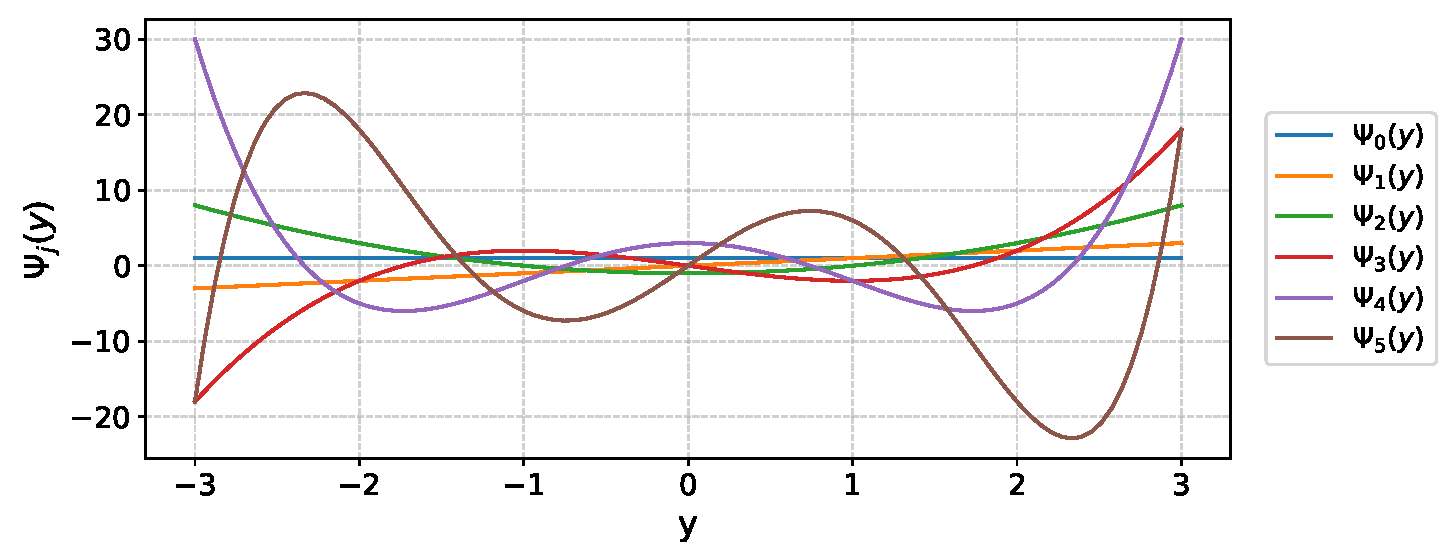
\includegraphics[width=\linewidth]{figures/Hermite.pdf}
    \caption{The first five Hermite polynomials evaluated over the real line.}
    \label{fig:hermite_polynomials}
\end{figure}

As illustrated in Figure~\ref{fig:hermite_polynomials}, the polynomials exhibit structural zero-crossings and growth rates that are well-suited for capturing the variations of a probability density. To parameterise the full multivariate transport map, we require multivariate basis functions. For the $k$-th component of the map, the function depends strictly on the first $k$ spatial coordinates, $x_1, \dots, x_k$, to enforce the lower-triangular structure of the Knothe-Rosenblatt rearrangement. We construct multivariate basis functions, $\Psi_j(x)$, by taking the tensor product of the univariate Hermite polynomials across these $k$ active dimensions. 

A full tensor product basis up to a maximum polynomial degree $D$ contains $(D+1)^k$ terms. For high-dimensional state spaces encountered in aerospace tracking problems, this exponential growth in decision variables renders the parameterisation computationally intractable. To alleviate this dimensionality issue, we enforce a priori mathematical sparsity through total degree truncation. We construct a filtered index set where a tensor product term is only retained if the sum of its univariate polynomial degrees is less than or equal to $D$. This truncation strategy limits the size of the basis while preserving the expressivity required to invert the physical nonlinear shears of the target distribution.

We denote the number of retained basis functions for the $k$-th map component as $J_k + 1$. We approximate the scalar map component using a linear combination of these basis functions:
\begin{equation}
    S^k(x) = \sum_{j=0}^{J_k} w_j^{(k)} \Psi_j(x),
    \label{eq:hermite_expansion}
\end{equation}
where the vector $w^{(k)} \in \mathbb{R}^{J_k+1}$ contains the unknown scalar coefficients that we must optimise. 

A direct mathematical advantage of this specific parameterisation emerges when evaluating the strict monotonicity constraint, $\partial_k S^k(x) > 0$. The derivative of a probabilist's Hermite polynomial obeys the linear relation:
\begin{equation}
    \frac{d}{dy} \mathrm{He}_m(y) = m \mathrm{He}_{m-1}(y).
    \label{eq:hermite_derivative}
\end{equation}
Because $\Psi_j(x)$ is a tensor product, the partial derivative $\partial_k$ only operates on the univariate polynomial associated with the $k$-th spatial coordinate, $x_k$. Consequently, the partial derivative of the map component reduces to a linear combination of lower-degree Hermite polynomials, evaluated strictly with respect to the decision variables $w^{(k)}$:
\begin{equation}
    \partial_k S^k(x) = \sum_{j=0}^{J_k} w_j^{(k)} \partial_k \Psi_j(x).
    \label{eq:map_derivative_linear}
\end{equation}
Substituting the finite expansion \eqref{eq:hermite_expansion} and its linear derivative \eqref{eq:map_derivative_linear} into the infinite-dimensional continuous objective \eqref{eq:mle_objective} reformulates the density estimation task as a finite-dimensional optimisation problem.